\documentclass[11pt]{article}
\usepackage[T1]{fontenc}
\usepackage[utf8]{inputenc}
\usepackage{amsmath,amssymb,amsthm,booktabs}
\usepackage[margin=1in]{geometry}
\usepackage{tikz}
\usetikzlibrary{arrows.meta,calc,positioning}
\usepackage{hyperref,xurl}
\hypersetup{colorlinks=true,linkcolor=blue!50!black,urlcolor=blue!50!black}
\newtheorem{theorem}{Theorem}[section]
\newtheorem{lemma}[theorem]{Lemma}
\newtheorem{proposition}[theorem]{Proposition}
\newtheorem{corollary}[theorem]{Corollary}
\theoremstyle{remark}
\newtheorem{remark}[theorem]{Remark}
\newcommand{\HH}{\mathbb H}
\newcommand{\Vol}{\operatorname{Vol}}
\newcommand{\ip}[2]{\langle #1,#2\rangle}
\newcommand{\OCT}{\mathcal O}
\newcommand{\DBL}{\mathcal D}
\newcommand{\CELL}{\mathcal C}
\title{Octahedral cuts and chains of ideal right-angled 24-cells}
\author{Coxeter Polytopes Research Project}
\date{18 October 2026; internal research manuscript}
\begin{document}
\maketitle
\begin{abstract}
We study a restricted class of finite-volume ideal right-angled
hyperbolic four-polytopes: every facet must be either a regular ideal
octahedron or the double of one across a triangular face. Inside each
doubled facet there is a distinguished ideal triangle. We show that
these triangles fit together into closed surfaces, and that every
connected surface consists of exactly eight triangles. Equal cusp
widths then put its triangles in one hyperplane and produce a regular
ideal octahedral section. Cutting along all such sections decomposes
the polytope into regular ideal 24-cells. An additional argument in
the $D_4$ root model forces the cells to form a chain, with consecutive
cuts opposite in each intermediate cell. The facet hypothesis is
essential: no classification of arbitrary ideal right-angled
four-polytopes or universal volume quantization is claimed. The proof
is written in full, with the geometric and topological reductions
separated from the finite model calculations. It is an internal
mathematical argument; external review and a complete Lean
formalization remain outstanding.
\end{abstract}

\section{The precise problem}

Let $\OCT$ be a regular ideal right-angled octahedron in $\HH^3$.
Reflect $\OCT$ across one triangular face and adjoin the reflected
copy. We denote the resulting ideal right-angled three-polyhedron
by $\DBL$. It has nine vertices, eight triangular faces and three
quadrilateral faces. Let $\CELL$ be the regular ideal right-angled
24-cell in $\HH^4$.

Throughout this paper, $P$ is a finite-sided, convex, finite-volume
four-polytope. Every vertex of $P$ is ideal and every dihedral angle
is $\pi/2$. We impose the additional condition
\begin{equation}\label{eq:spectrum}
 \text{every facet of $P$ is isometric to $\OCT$ or $\DBL$.}
\end{equation}
The word ``isometric'' fixes the intrinsic geometry of the facets,
not merely their face counts. One can instead assume the corresponding
combinatorial types and invoke the usual three-dimensional
right-angled rigidity, but no such classification is needed once
\eqref{eq:spectrum} is part of the hypothesis.

\begin{theorem}\label{thm:main}
Suppose that $P$ satisfies \eqref{eq:spectrum}. There are finitely many
pairwise disjoint regular ideal octahedral sections which cut $P$ into
regular ideal right-angled 24-cells. If $P$ has $N$ facets of type
$\DBL$, then $N=8k$ for some integer $k\ge0$, and there are $k+1$
cells in the decomposition. Their adjacency graph is a path.
In every cell incident to two cuts, the two cutting facets are opposite.
Consequently, within the class \eqref{eq:spectrum}, the isometry type
of an existing polytope is determined by its number of cells, and
\[
 \Vol(P)=(k+1)\frac{4\pi^2}{3}.
\]
\end{theorem}

The last assertion classifies existing polytopes in this restricted
class; we do not use it to assert existence for every prescribed path
length. In particular, Theorem~\ref{thm:main} is not a proof that every
ideal right-angled four-polytope is a chain of 24-cells. Its role is to
identify exactly how far the octahedral cutting argument extends
without allowing more complicated facets.

The proof has two distinct stages. We first build a cutting section
from intrinsic facet geometry. We then control the arrangement of
the sections inside the resulting 24-cells. Neither stage assumes
that the polytope was constructed by gluing cells.

\section{What a doubled facet contributes at a cusp}

The three vertices of the gluing face of $\DBL$ have a simple
intrinsic description: their horospherical rectangles are nonsquare.
At each of these vertices the rectangle is obtained by adjoining
two unit squares along one side, and therefore has aspect ratio two.
The remaining six rectangles are square. The three quadrilateral
faces of $\DBL$ meet pairwise at its three nonsquare cusps and have
no common edges. At a nonsquare cusp, the two quadrilateral sides
are the two long sides of its $2$ by $1$ rectangle.

The convex hull of the three nonsquare cusps is an ideal triangle
$T_F$ whose relative interior lies in the relative interior of a
doubled facet $F$. This is its
original gluing triangle. Each side of $T_F$ is the interior diagonal
of a quadrilateral face of $F$. At a nonsquare cusp, $T_F$ meets
the horospherical rectangle along the transverse segment halfway
along its long direction. Figure~\ref{fig:rectangle} records these
facts in the Euclidean link, where their metric meaning is literal.

\begin{figure}[htbp]
\centering
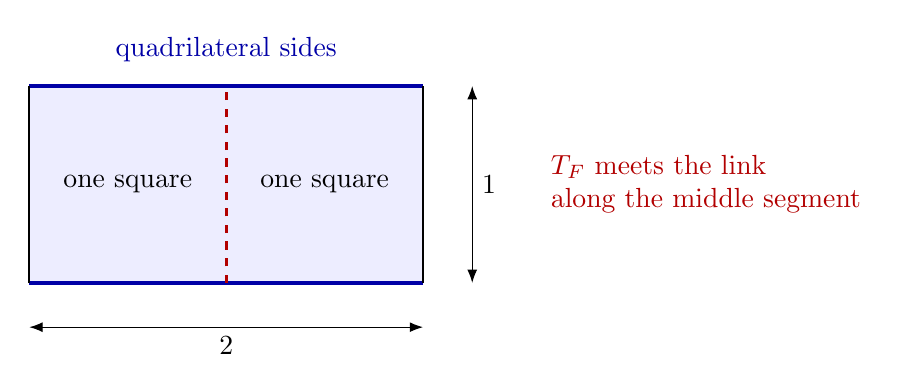
\begin{tikzpicture}[scale=1.25,>=Latex]
 \fill[blue!7] (0,0) rectangle (4,2);
 \draw[very thick,blue!65!black] (0,0)--(4,0) (0,2)--(4,2);
 \draw[thick] (0,0)--(0,2) (4,0)--(4,2);
 \draw[dashed,very thick,red!70!black] (2,0)--(2,2);
 \draw[<->] (0,-.45)--node[below] {$2$}(4,-.45);
 \draw[<->] (4.5,0)--node[right] {$1$}(4.5,2);
 \node at (1,1) {one square};
 \node at (3,1) {one square};
 \node[above,blue!65!black] at (2,2.15) {quadrilateral sides};
 \node[align=left,anchor=west,red!70!black] at (5.2,1)
 {$T_F$ meets the link\\along the middle segment};
\end{tikzpicture}
\caption{The cusp rectangle of a doubled octahedron at a gluing
vertex. The blue sides belong to its quadrilateral faces. The red
segment is the link of the internal triangle. This is an exact
Euclidean link diagram, not a perspective drawing of $\HH^4$.}
\label{fig:rectangle}
\end{figure}

At a square cusp of $\DBL$, exactly one incident polygonal face
is a quadrilateral. At a cusp of $\OCT$, none is. These two small
incidence facts will exclude one possible ambient box shape.

\begin{lemma}\label{lem:box}
Every noncubic cusp box of $P$ has side proportions $2:1:1$.
Its four nonsquare faces belong to doubled facets and form a belt;
its two square end faces belong to ordinary octahedral facets.
Every adjacency within the belt is a quadrilateral ridge of $P$.
\end{lemma}
\begin{proof}
Each face rectangle of a cusp box is intrinsic to a facet of $P$.
Its aspect ratio is therefore one or two. If the three side lengths
were distinct, the ratio of the largest to the smallest would exceed
two, since the two consecutive unequal ratios must both be two.
Thus a noncubic box has proportions $2:1:1$ or $2:2:1$.

Consider a $2:2:1$ box. The four nonsquare faces must be doubled
facets. In each, the two long sides are quadrilateral sides. Each
square end face consequently has four incident quadrilateral sides.
An octahedral cusp has none, and a square cusp of a doubled facet
has exactly one. Neither permitted facet type can supply an end
face. The $2:2:1$ box is impossible.

In a $2:1:1$ box, the four long rectangles are the belt. Their
mutual sides are the long sides and hence are quadrilateral ridges.
The square ends meet the belt only along its short, triangular
sides. All four incidences at an end are triangular, so the end
cannot be a square cusp of a doubled facet. It is octahedral.
\end{proof}

\section{The internal triangles form closed surfaces}

Join two doubled facets when they share a quadrilateral ridge.
The distinguished triangles in these facets have the same internal
diagonal in that ridge, so we glue them along this diagonal. The
gluing is geometrically defined; there is no choice of an abstract
edge identification.

\begin{lemma}\label{lem:surface}
After adjoining their ideal vertices, the glued triangles form a
finite closed two-manifold. Its connected components are exactly
the components of the quadrilateral adjacency graph of doubled facets.
Every edge lies in two triangles and every vertex lies in four.
\end{lemma}
\begin{proof}
The interior of a distinguished triangle lies in the relative
interior of its facet. Interiors of different facets are disjoint.
An edge of the triangle is in the relative interior of an actual
quadrilateral ridge, which lies in precisely two facets. Thus each
edge has two incident triangles and has a disk neighborhood at
each of its finite points.

It remains to check the ideal vertices. By Lemma~\ref{lem:box},
the triangles incident to one such point come from the four doubled
facets in a single $2:1:1$ belt. Their four middle segments join
end to end around the box, giving the simple square shown in
Figure~\ref{fig:belt}. They do not cross and do not leave an open
end. This square is the link of the point in the glued surface.
Coning the link gives a disk after the ideal point is adjoined.
There are no other triangle vertices.

All four doubled facets at such a vertex are already connected
through their quadrilateral belt. Therefore identifying ideal
vertices does not join two different components of the quadrilateral
adjacency graph. The components of the graph and of the surface
coincide.
\end{proof}

\begin{figure}[htbp]
\centering
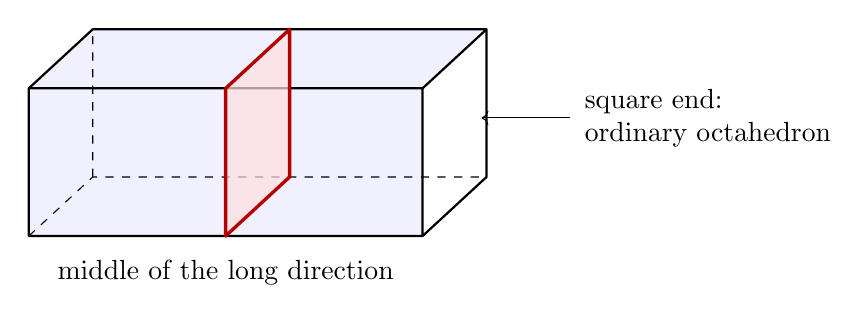
\begin{tikzpicture}[scale=1.25,line join=round]
 \coordinate (A) at (0,0); \coordinate (B) at (4,0);
 \coordinate (C) at (4,1.5); \coordinate (D) at (0,1.5);
 \coordinate (E) at (.65,.6); \coordinate (F) at (4.65,.6);
 \coordinate (G) at (4.65,2.1); \coordinate (H) at (.65,2.1);
 \fill[blue!6] (A)--(B)--(C)--(G)--(H)--(D)--cycle;
 \draw[thick] (A)--(B)--(C)--(D)--cycle (B)--(F)--(G)--(C)
 (D)--(H)--(G);
 \draw[dashed] (A)--(E)--(F) (E)--(H);
 \fill[red!12,opacity=.7] (2,0)--(2.65,.6)--(2.65,2.1)--(2,1.5)--cycle;
 \draw[very thick,red!70!black] (2,0)--(2.65,.6)--(2.65,2.1)--(2,1.5)--cycle;
 \node[below] at (2,-.15) {middle of the long direction};
 \draw[->] (5.5,1.2)--(4.6,1.2);
 \node[anchor=west,align=left] at (5.55,1.2)
 {square end:\\ordinary octahedron};
\end{tikzpicture}
\caption{Four internal triangles meet an ambient $2:1:1$ cusp box
in its transverse middle square. Its boundary is the four-segment
link used to prove that the compactified triangle complex is a
two-manifold. The filled square indicates the transverse section;
only its boundary lies on the box surface.}
\label{fig:belt}
\end{figure}

\begin{lemma}\label{lem:euler}
A connected component containing $n$ triangles contains exactly
eight triangles, twelve edges and six vertices.
\end{lemma}
\begin{proof}
Write $e$ and $v$ for its edge and vertex counts. The incidence
counts of Lemma~\ref{lem:surface} give
\[
 e=\frac{3n}{2},\qquad v=\frac{3n}{4},\qquad
 \chi=v-e+n=\frac n4.
\]
We shall use only the elementary inequality $\chi\le2$ for a
connected closed cellulated surface; we do not assume the surface
is a sphere. Here is a direct proof in the present setting.
Choose a spanning tree $A$ of its one-skeleton. Delete from the
dual graph the edges dual to $A$. The remaining dual graph is
connected. Otherwise, the boundary between one nonempty proper
set of triangular faces and its complement would be a nonempty
subgraph of $A$. At each vertex its degree is even: a walk around
the circular link enters and leaves the chosen set equally often.
This gives a nonempty Eulerian subgraph of a tree, which is
impossible. We may therefore choose a dual spanning tree disjoint
from $A$. The two trees use $v-1$ and $n-1$ distinct edges, so
$e\ge v+n-2$ and $\chi\le2$. It follows that $n\le8$, and the
integer $\chi=n/4$ also shows that $n$ is divisible by four.

We next obtain a lower bound within the same component. Choose
one doubled facet $F$. Its three quadrilateral faces have three
distinct doubled neighbors. Its three nonsquare cusps also have
three opposite doubled facets. The latter are distinct from one
another and from every ridge neighbor: their walls are asymptotic
to the wall of $F$ at exactly one specified ideal point, whereas
a ridge neighbor intersects its wall along a plane. These opposite
facets belong to the same component, because opposite belt members
are connected by the four-cycle of quadrilateral adjacencies.
Together with $F$ we have found seven distinct facets in the
component. Thus $7\le n\le8$ and $4\mid n$, forcing $n=8$.
The values of $e$ and $v$ follow.
\end{proof}

\section{From six cusps to eight wall normals}

Fix one component. Make a graph $J$ whose six vertices are its
cusps and whose edges are the twelve internal diagonals. Every
vertex has degree four.

\begin{lemma}\label{lem:graph}
The graph $J$ is the octahedral graph. Its eight triangles are the
eight distinguished facet triangles. The doubled facets can
therefore be indexed by $s\in\{\pm1\}^3$ so that quadrilateral
adjacency changes exactly one sign.
\end{lemma}
\begin{proof}
First, $J$ has no parallel edges. If two different quadrilateral
ridges joined the same two cusps, their incident facets would
include at least three of the four belt members at either cusp.
Among three belt members there are two opposite ones. Their walls
are asymptotic at that cusp and cannot contain the second cusp.
This is a contradiction. Two distinct ridges cannot have the same
pair of incident facets, since the intersection of two convex
facets is one face. Thus $J$ is simple.

A simple four-regular graph on six vertices has complement a
perfect matching, so it is the octahedral graph. Each distinguished
triangle gives a three-cycle in $J$. Two facets cannot give the
same three-cycle: its geometric triangle would then have an
interior point in the relative interiors of two different facets.
The octahedral graph has exactly eight three-cycles, obtained by
choosing one vertex from each of its three opposite pairs. All
eight occur. Label these opposite pairs by $1,2,3$, with a sign
on each member. A triangle, and hence a doubled facet, is indexed
by its three choices of sign. Two triangles share an edge exactly
when one sign changes.
\end{proof}

\begin{figure}[htbp]
\centering
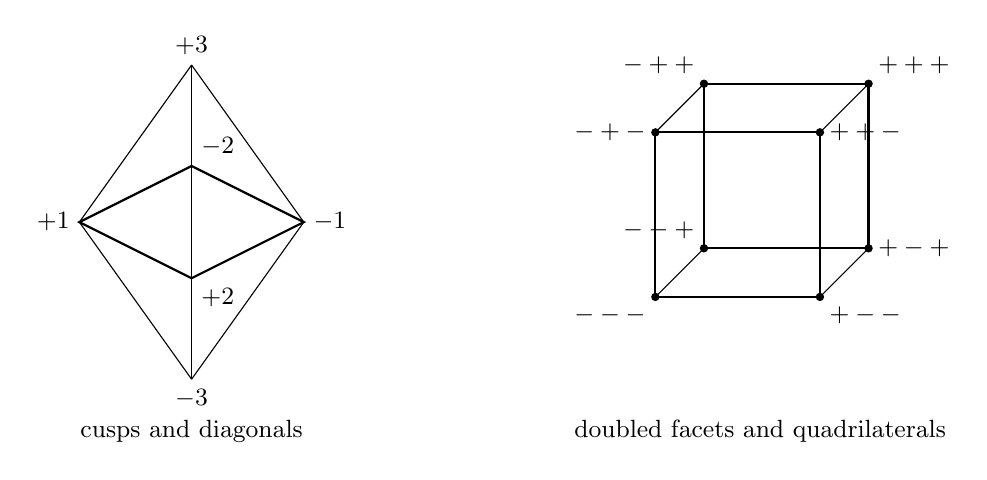
\begin{tikzpicture}[scale=.95,every node/.style={font=\small}]
 \coordinate (xp) at (-1.5,0); \coordinate (yp) at (0,-.75);
 \coordinate (xm) at (1.5,0); \coordinate (ym) at (0,.75);
 \coordinate (zp) at (0,2.1); \coordinate (zm) at (0,-2.1);
 \draw[thick] (xp)--(yp)--(xm)--(ym)--cycle;
 \foreach \p in {xp,yp,xm,ym}{\draw (zp)--(\p) (zm)--(\p);}
 \node[left] at (xp) {$+1$}; \node[right] at (xm) {$-1$};
 \node[below right] at (yp) {$+2$}; \node[above right] at (ym) {$-2$};
 \node[above] at (zp) {$+3$}; \node[below] at (zm) {$-3$};
 \node at (0,-2.8) {cusps and diagonals};
 \begin{scope}[xshift=6.2cm,yshift=-1cm]
 \coordinate (a) at (0,0); \coordinate (b) at (2.2,0);
 \coordinate (c) at (2.2,2.2); \coordinate (d) at (0,2.2);
 \coordinate (e) at (.65,.65); \coordinate (f) at (2.85,.65);
 \coordinate (g) at (2.85,2.85); \coordinate (h) at (.65,2.85);
 \draw[thick] (a)--(b)--(c)--(d)--cycle (e)--(f)--(g)--(h)--cycle;
 \draw (a)--(e) (b)--(f) (c)--(g) (d)--(h);
 \foreach \p/\lab/\pos in {a/{---}/below left,b/{+--}/below right,
 c/{++-}/right,d/{-+-}/left,e/{--+}/above left,f/{+-+}/right,
 g/{+++}/above right,h/{-++}/above left}
 {\fill (\p) circle (1.6pt);\node[\pos] at (\p) {$\lab$};}
 \node at (1.4,-1.8) {doubled facets and quadrilaterals};
 \end{scope}
\end{tikzpicture}
\caption{The two incidence graphs. The six-cusp graph is octahedral;
its eight triangles index the doubled facets. The dual cube records
quadrilateral adjacency. The signs specify which cusp from each
opposite pair belongs to a distinguished triangle. These are
incidence drawings, not metric projections of the polytope.}
\label{fig:graphs}
\end{figure}

\section{Equal widths put the triangles in one hyperplane}

We work in $\mathbb R^{4,1}$ with form
$\ip{x}{x}=-x_0^2+x_1^2+\cdots+x_4^2$. A wall has an outward
unit spacelike normal $n$, and its halfspace is $\ip{x}{n}\le0$.
Let $n_s$ be the normals of the eight doubled facets just indexed.

\begin{lemma}\label{lem:width}
On each square of the cube in Figure~\ref{fig:graphs}, the sums of
the two opposite pairs of normals agree.
\end{lemma}
\begin{proof}
The square is a cusp belt. Its opposite wall pairs bound the two
short directions of the $2:1:1$ box, so their Euclidean separations
on a common horosphere agree. The use of unit normals matters.
With cusp null vector $\xi=(1,0,0,0,1)$, the vertical wall $x_i=a$
in upper-half-space has unit normal $(a,e_i,a)$. The opposite wall
$x_i=b$, with the other outward orientation, has normal
$(-b,-e_i,-b)$. Their sum is $(a-b)\xi$. Thus its coefficient is
the separation, with the same normalization for both pairs. Equal
widths give equal sums.
\end{proof}

\begin{lemma}\label{lem:normal}
There are mutually orthogonal vectors $a,b_1,b_2,b_3$ such that
\[
 n_s=a+s_1b_1+s_2b_2+s_3b_3,\qquad
 a^2=-\tfrac12,\quad b_i^2=\tfrac12.
\]
\end{lemma}
\begin{proof}
The equations of Lemma~\ref{lem:width} say that every mixed second
finite difference on the cube vanishes. Expanding $s\mapsto n_s$
in sign characters leaves only its constant and three linear
terms, giving the displayed affine expression. Expanding the
eight equations $n_s^2=1$ and comparing sign characters gives
\[
 \ip{a}{b_i}=0,\quad \ip{b_i}{b_j}=0\ (i\ne j),\quad
 a^2+b_1^2+b_2^2+b_3^2=1.
\]
Adjacent facets meet orthogonally. If $s'$ differs from $s$ only
in coordinate $i$, then
$0=\ip{n_s}{n_{s'}}=1-2b_i^2$. Thus every $b_i^2=1/2$, and
the remaining identity gives $a^2=-1/2$.
\end{proof}

The span $U$ of these four vectors is Lorentzian and has dimension
four. Its orthogonal complement is a spacelike line. The
intersection of $U$ with $\HH^4$ is a genuine hyperbolic
hyperplane $H$, orthogonal to all eight doubled-facet walls.
In orthonormal coordinates on $U$, the wall normals are
$(1,s_1,s_2,s_3)/\sqrt2$, with the future sign determined by their
positive cusp-null sums. Their halfspaces cut out
\begin{equation}\label{eq:section}
 S=\{(t,x)\in\HH^3:|x_1|+|x_2|+|x_3|\le t\},
\end{equation}
the regular ideal octahedron. Its six null rays are $a\pm b_i$.
They are exactly the actual cusps of the component, because the
opposite belt-normal sums are $2(a\pm b_i)$.

Convexity now supplies the step that an abstract graph cannot:
since these six ideal points belong to the closure of $P$, their
hyperbolic convex hull $S$ is contained in $P$. Conversely the
eight actual facet inequalities imply $P\cap H\subset S$.
Therefore
\[
 P\cap H=S.
\]
Each face of $S$ is its facet's distinguished internal triangle.
Each edge of $S$ is the internal diagonal of an actual
quadrilateral ridge, as illustrated in Figure~\ref{fig:diagonal}.

\begin{figure}[htbp]
\centering
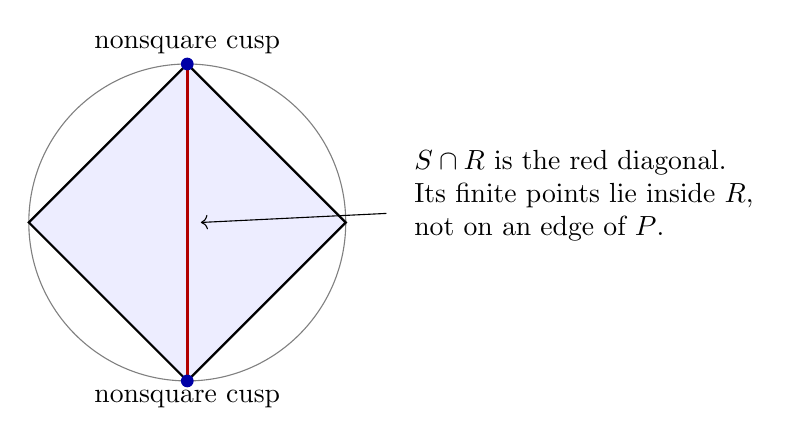
\begin{tikzpicture}[scale=1.15]
 \draw[gray] (0,0) circle (1.75);
 \coordinate (a) at (0,1.75); \coordinate (b) at (1.75,0);
 \coordinate (c) at (0,-1.75); \coordinate (d) at (-1.75,0);
 \fill[blue!7] (a)--(b)--(c)--(d)--cycle;
 \draw[thick] (a)--(b)--(c)--(d)--cycle;
 \draw[very thick,red!70!black] (a)--(c);
 \fill[blue!65!black] (a) circle (2pt) (c) circle (2pt);
 \node[above] at (a) {nonsquare cusp};
 \node[below] at (c) {nonsquare cusp};
 \node[anchor=west,align=left] at (2.4,.3)
 {$S\cap R$ is the red diagonal.\\Its finite points lie inside $R$,\\
 not on an edge of $P$.};
 \draw[->] (2.2,.1)--(.15,0);
\end{tikzpicture}
\caption{A quadrilateral ridge $R$ in the Klein disk. Its two
nonsquare cusps are opposite vertices. Their diagonal is an edge
of the cutting octahedron. This distinction is what prevents an
unrelated facet from touching the section at a finite edge point.}
\label{fig:diagonal}
\end{figure}

\section{Why the hyperplane is a legitimate cut}

\begin{lemma}\label{lem:cut}
No facet outside the chosen eight meets $S$ at a finite point.
Cutting along $H$ gives two finite-volume entirely ideal
right-angled four-polytopes. The eight doubled facets become
ordinary octahedra; every other facet is uncut.
\end{lemma}
\begin{proof}
Let $F$ be any outside facet. Its supporting functional is
nonpositive on $S$. If it vanishes at a relative interior point
of a face of $S$, it vanishes on that face. A finite point of $S$
lies in its interior, in a triangular face interior, or in an
edge interior. A triangular face interior belongs to the relative
interior of one of the chosen doubled facets, so it cannot belong
to $F$. An edge interior lies in the relative interior of a ridge
whose only two incident facets are the chosen doubled facets.
It cannot belong to $F$ either. A supporting functional vanishing
at an interior point would contain all of $S$, contradicting the
face-interior case. Thus $F$ has no finite intersection with $S$.

If $F$ crossed $H$, a finite segment in $F$ would meet
$P\cap H=S$ at a finite point. Consequently no outside facet
crosses. The chosen eight facets are cut along their genuine
gluing triangles into octahedra. The center of $S$ is strict on
all eight wall inequalities and, by what was just proved, on
every other wall inequality. It is an interior point of $P$;
both halves have nonempty interior.

In the Klein model, a vertex of a half lying on $H$ must be a
vertex of $S$. Otherwise it lies in a nontrivial segment of $S$
and is not extreme. Away from $H$, a vertex is an old vertex of
$P$. The only vertices of $S$ are its six old ideal cusps, so
no finite vertex is introduced. The new facet $S$ meets only the
eight cut walls, all orthogonal to $H$. Every new dihedral angle
is right; all other angles are inherited. Finite volume follows
by containment in $P$.
\end{proof}

The facet spectrum \eqref{eq:spectrum} is preserved by the cut.
There are exactly eight fewer doubled facets, counted over both
pieces. Repeating the construction therefore terminates.

There is also a useful geometric disjointness statement. Every
outside doubled facet lies on one side of the first cut. Two
quadrilateral-adjacent outside facets cannot lie on opposite
sides, since their shared ridge would give a finite intersection
with $S$. Thus a whole other component lies on one side. Its
section, being the convex hull of its six cusps, lies on that
side as well. A noncubic cusp belongs to only one belt component
and has octahedral ends; two sections cannot share an ideal
vertex. The outside-facet argument excludes finite boundary
contact. Hence the sections are pairwise disjoint, including
their ideal endpoints.

\section{Recognizing a piece with only octahedral facets}

We give a direct recognition argument rather than using a
four-dimensional classification as a final black box.

\begin{lemma}\label{lem:recognition}
An entirely ideal right-angled four-polytope whose facets are all
isometric to $\OCT$ is isometric to $\CELL$.
\end{lemma}
\begin{proof}
Place one facet $F$ on a facet of a model regular 24-cell. Its
eight triangular faces agree with those of the model facet.
For any one of these triangles, the adjacent supporting wall is
uniquely determined by the triangle and orthogonality to $F$'s
wall: its outward normal is the intrinsic outward unit normal
of that triangle within $F$'s wall.

In this adjacent wall, its octahedral facet is determined by the
shared ideal triangle and the side on which it lies. To justify
this last assertion, take any isometry between two regular ideal
octahedra with that triangular face. Every isometry of the face
extends to a symmetry of the octahedron, so the isometry can be
adjusted to fix the face vertices pointwise. An isometry of
$\HH^3$ fixing three distinct ideal points is the identity or
reflection in their plane; the specified side selects the
identity. The neighboring facet is therefore the whole model
octahedron, not only a piece on the same wall.

Repeat across its faces. The facet adjacency graph of the model
24-cell is connected. The propagation matches all 24 model
facets, with their full vertex sets, to actual facets of the
piece. Their halfspaces put the piece inside the model cell.
Conversely the closure of the piece contains every ideal model
vertex, and convexity contains their hull, the model cell.
The two polytopes agree.
\end{proof}

Each final piece is consequently a 24-cell. If the original
polytope has $N$ doubled facets, Lemma~\ref{lem:euler} gives
$N=8k$. Each of the $k$ cuts increases the number of pieces by
one, so there are $k+1$ cells. Their adjacency graph is a tree:
starting with one piece, each separating cut replaces one vertex
of the current adjacency tree by two vertices joined by one edge.

\section{Why the tree is a chain}

The restriction on facet types has one more consequence. In the
Lorentz model a regular 24-cell has outward unit normals
\[
 (1,r),\qquad
 r\in\{(\pm1,\pm1,0,0)\text{ and all coordinate permutations}\}.
\]
The spatial vectors are the roots of $D_4$. Distinct roots have
dot products $-2,-1,0,1$, with $-2$ only for opposite roots.

\begin{lemma}\label{lem:opposite}
If a cell in the decomposition meets two cutting sections,
these are opposite facets of that cell.
\end{lemma}
\begin{proof}
The sections have disjoint closures. If their roots are $r_1,r_2$,
then $r_1\cdot r_2$ is negative: dot product one gives an actual
common triangular ridge, and dot product zero gives a common
ideal vertex. Thus the dot product is $-1$ or $-2$.

Suppose it is $-1$. The vector $r_1+r_2$ is another $D_4$ root,
and its cell facet $Q$ is orthogonal to both cut walls, since
\[
 -1+(r_1+r_2)\cdot r_i=0\qquad(i=1,2).
\]
It cannot itself be a cutting facet, since it meets the two
sections along triangles. It is part of an original facet of $P$.
Across each of the two cuts there is a neighboring regular
24-cell. Its corresponding facet is the reflection of $Q$ and
lies in the same original supporting wall, because that wall is
orthogonal to the cut. This neighboring facet cannot be another
internal cut: it meets the first cut along a triangle, whereas
all cuts have disjoint closures. Thus the original facet contains
three regular ideal octahedra.

Their relative interiors are disjoint. If two had an open
overlap, a point of that overlap avoiding every other cell wall
would have an inward normal collar contained in both cells.
Their four-dimensional interiors would overlap, which is
impossible for pieces obtained by cuts. The original facet has
intrinsic volume at least three times $\Vol(\OCT)$; it can be
neither $\OCT$ nor $\DBL$. This contradicts
\eqref{eq:spectrum}. Hence the dot product is $-2$, and the two
facets are opposite.
\end{proof}

No cell can have three pairwise opposite facets. The adjacency
tree has maximum degree two and is a path. Once an end cell and
its first gluing facet are placed, every next cell is its
reflection across the gluing facet, and the next gluing facet in
an intermediate cell is uniquely the opposite one.

For completeness, there is no independent gluing twist. The
regular 24-cell is flag-transitive. Given an isometry of an
octahedral facet, send one facet flag to its image by a cell
symmetry. This symmetry stabilizes the facet and has the required
restriction, because an octahedral isometry fixing a flag is the
identity. Thus every facet symmetry extends to the cell.
Two cells on opposite sides of the same facet are therefore
uniquely placed up to the ambient reflection. This proves the
isometry assertion in Theorem~\ref{thm:main}.

\begin{figure}[htbp]
\centering
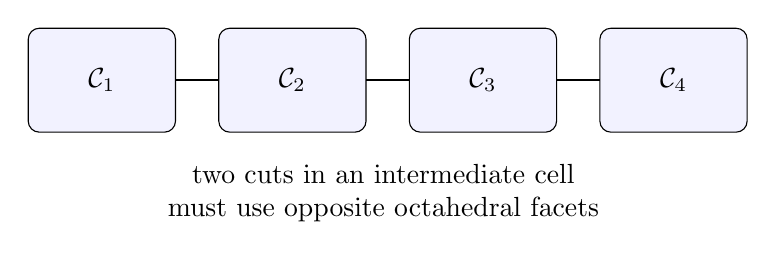
\begin{tikzpicture}[>=Latex,scale=1.1]
 \foreach \i in {0,1,2,3}{
  \draw[rounded corners,fill=blue!5] (2.2*\i,0) rectangle +(1.7,1.2);
  \node at (2.2*\i+.85,.6) {$\CELL_{\the\numexpr\i+1\relax}$};}
 \foreach \i in {0,1,2}{\draw[thick] (2.2*\i+1.7,.6)--(2.2*\i+2.2,.6);}
 \node[align=center] at (4.1,-.7)
 {two cuts in an intermediate cell\\must use opposite octahedral facets};
\end{tikzpicture}
\caption{The resulting adjacency graph is a path. The boxes denote
whole 24-cells and are not metric four-dimensional drawings. The
opposition condition comes from the common-neighbor argument in
Lemma~\ref{lem:opposite}, rather than from the drawing.}
\label{fig:chain}
\end{figure}

\section{Volume, face counts, and the limit of the result}

The regular ideal 24-cell has volume $4\pi^2/3$.
Volume additivity proves the formula in the main theorem. There
is a second way to see the same integer. Write $v,e,r,f$ for
the face counts of $P$ and put
\[
 W=\sum_{R}(k(R)-3),
\]
where $k(R)$ is the number of vertices of a ridge. Cusp-box
incidence and Euler's equation give
\[
 e=4v,\quad r=3v+f,\quad W=3(v-f).
\]
An octahedral facet has defect zero and a doubled facet defect
three, where the defect is the sum of $k(R)-3$ over its faces.
Every ridge is counted twice, so $2W=3N=24k$. The volume formula
\cite[Lemma~2]{Kolpakov} therefore gives
\[
 \Vol(P)=\frac{4\pi^2}{3}+\frac{\pi^2}{9}W
 =(k+1)\frac{4\pi^2}{3}.
\]

If there are $m=k+1$ cells, the complete face counts are
\[
 (v,e,r,f)=(18m+6,\ 72m+24,\ 68m+28,\ 14m+10).
\]
Indeed each gluing identifies six ideal vertices and removes two
facets while merging eight neighboring pairs. There are no extra
vertex identifications between nonadjacent cells: a common cusp
would lie on every separating cut along their path, whereas
different sections have no common ideal vertex. The edge and
ridge formulas then follow from the incidence identities above.
There are $8(m-1)$ doubled facets, $6m+18$ ordinary facets and
$12(m-1)$ quadrilateral ridges. All other ridges are triangles.
For $m=2$ this recovers $(42,168,164,38)$.

These formulas do not establish the same quantization for arbitrary
ideal right-angled four-polytopes. Without
\eqref{eq:spectrum}, a facet may have more complicated cusp
rectangles, the internal triangles used here may not exist, and
the local links need not be the four-segment belts of
Lemma~\ref{lem:surface}. A successful extension must replace those
geometric facts, not merely repeat the Euler count.

\appendix
\section{Proof inputs and verification status}

The geometric inputs are the explicit regular octahedron, its
double, the regular 24-cell, the rectangular link of an ideal
right-angled cusp, and the usual Lorentz description of supporting
walls. The surface Euler bound, cusp-component injection, six-cusp
graph, normal equations, actual cutting argument, all-octahedral
recognition and opposition argument are proved in this manuscript.
The volume formula is cited for the alternative computation; the
decomposition and volume-additivity argument do not depend on a
published volume-minimum classification.

The written decomposition proof has a separate internal mathematical
review. The stronger opposition argument is subject to its own review
record. Existing exact local certificates check the octahedron-double
cusp data and cube-normal algebra; they do not certify the universal
surface construction or convexity arguments. No end-to-end Lean
verification or external human review is claimed. Build records and
the precise review links belong to the reproduction document, rather
than serving as mathematical premises here.

\begin{thebibliography}{9}
\bibitem{Kolpakov}
A.~Kolpakov, \emph{On the optimality of the ideal right-angled 24-cell},
Algebraic \& Geometric Topology \textbf{12} (2012), 1941--1960.
\href{https://doi.org/10.2140/agt.2012.12.1941}{doi:10.2140/agt.2012.12.1941}.
\end{thebibliography}
\end{document}
